\section{Evaluation der integrierten Erklärungen}

Um die vorgestellten Erklärungen für \textit{NUNAV Navigation} auf die Erfüllung der aufgestellten Ziele zu überprüfen wurde anhand des entwickelten Leitfadens eine Studie zur Evaluation der Erklärungen entworfen. Außerdem sind die Ergebnisse aus dem durchgeführten Workshop mit in das Studiendesign eingeflossen (siehe \nameref{ch:appendix_1}). Die Studie ist in zwei Teile gegliedert. Im ersten Teil ist eine \textit{Case Study} \cite{wohlin2012experimentation} durchgeführt worden, welche in die Produktivversion von \textit{NUNAV Navigation} integriert wurde. Um die Ergebnisse daraus besser einordnen zu können, ist im Anschluss daran mit vier Nutzern, die in der vorherigen Studie nicht teilgenommen haben, ein Quasi-Experiment [wohlin2012experimentation] durchgeführt worden.

\subsection{Ziel der Evaluation}

Das Ziel der Evaluation ist wie auch das Ziel der gesamten Arbeit (siehe \autoref{sec:goal_definition}) auf Basis der Vorlage von \citeauthor{wohlin2012experimentation} formuliert \cite{wohlin2012experimentation}.

\smallskip

\noindent\fbox{
    \parbox{0.964\textwidth}{
        \smallskip
        Die Studie \textbf{analysiert} die integrierten Erklärungen \textbf{in Bezug auf} die externe Qualität des Systems \textbf{zur} Evaluation \textbf{aus der Sicht} von \textit{End Usern} \textbf{im Kontext} der Benutzung von \textit{NUNAV Navigation}.
        \smallskip
    }
}

\smallskip

Dem zu Folge sollte im Rahmen der Evaluation überprüft werden, ob die zuvor aus den abgeleiteten Zielen von \textit{Graphmasters} definierten Qualitätsanforderungen durch die entwickelten Erklärungen erfüllt werden können.

\subsubsection{Hypothesen}
\label{sec:evaluation_hypothesis}

Die Überprüfung der Erfüllung der gestellten Qualitätsanforderungen erfolgt im Rahmen von Hypothesentests \cite{wohlin2012experimentation}. Grundsätzlich wurden zwei abstrakte Einflusshypothesen für die Integration der Erklärungen aufgestellt:

\begin{itemize}
    \item WENN die Studienteilnehmer Erklärungen erhalten, DANN ist ein positiver Einfluss auf die externe Softwarequalität messbar im Vergleich zu Teilnehmern, welche keine Erklärungen erhalten.
    \item WENN die Studienteilnehmer mehrere Erklärungen erhalten, DANN ist ein positiver Einfluss auf die externe Softwarequalität messbar im Vergleich zu Teilnehmern, welche nur eine Erklärung erhalten.
\end{itemize}

\subsection{Studienaufbau}

Ein Ergebnis des durchgeführten Workshops war, dass die Erklärungen nach Möglichkeit unter Realbedingungen evaluiert werden sollen. Daraus ist die Anforderung abgeleitet worden, dass eine Studie die \textit{End User} von \textit{NUNAV Navigation} so wenig wie möglich bemerken sollten. Daher kommen lediglich Verhaltensmetriken oder bereits in der Anwendung integrierte Metriken zum Einsatz.

Die genutzten Metriken wurden aus dem \autoref{sec:explanation_requirements} zur Definition der Anforderungen übernommen und sind bereits vor Beginn dieser Arbeit in \textit{NUNAV Navigation} integriert gewesen.

Aufgrund von Einflusshypothesen durch Störgrößen wurden neben den Erklärungsmetriken zusätzliche Metriken in die Anwendung integriert. Das Ziel dabei war es, auf der Basis möglicher Einflüsse Datensätze herausfiltern zu können, welche die Ergebnisse der Analyse der Einflüsse durch integrierte Erklärungen zu verzerren (siehe \autoref{sec:evaluation_other_dependencies}).

\subsection{Studiendurchführung}

Insgesamt wurde folglich eine zwei-wöchige Case Study als empirische Strategie gewählt. Um die Unterschiede in Bezug auf die externe Qualität messen zu können, wurden nicht allen Teilnehmern die Erklärungen angezeigt. Zusätzlich sollte nicht nur eine Veränderung durch die Erklärungen messbar gemacht werden, sondern auch zwischen den einzelnen entwickelten Erklärungen unterschieden werden. Trotz dessen sollte auch die Kombination der verschiedenen Erklärungen überprüft werden. Um jedoch für jede Bedingung genug Nutzer als Datengrundlage zu haben, wurden nicht alle verschiedenen Kombinationsmöglichkeiten der Erklärungen überprüft.

Grundsätzlich wurden die Erklärungen in die zwei Gruppen \textit{statische} und \textit{Context}-abhängige Erklärungen gegliedert. Unter den statischen Erklärungen sind die beiden Erklärungen, welche den Routingalgorithmus und die Einflüsse auf die Routenberechnung erklären, zusammengefasst (siehe \autoref{sec:explanation_design}).

Analog dazu sind die \textit{Context}-Erklärungen zum aktuellen Verkehrsaufkommen und zu Positionsungenauigkeiten während der Navigation als eine Bedingung für die Studie zusammengefasst worden (siehe \autoref{sec:traffic_volume_definition} und \autoref{sec:gps_accuracy_definition}).

Insgesamt sind folglich vier verschiedene Studiengruppen entstanden:

\begin{itemize}
    \item \textbf{Gruppe 1}: Nutzer, die keine Erklärungen erhalten
    \item \textbf{Gruppe 2}: Nutzer, die statische Erklärungen erhalten
    \item \textbf{Gruppe 3}: Nutzer, die \textit{Context}-abhängige Erklärungen erhalten
    \item \textbf{Gruppe 4}: Nutzer, die statische als auch \textit{Context}-abhängige Erklärungen erhalten
\end{itemize}

Für die Zuordnung der einzelnen Studiengruppen wurde das im Rahmen dieser Arbeit entwickelte \textit{Feature-Flag}-System verwendet. Anhand von zufällig generierten Identifikatoren wurde zu diesem Zweck ein Hashwert berechnet und die Teilnehmer anhand der Teilbarkeit durch vier, den einzelnen Gruppen zugeordnet (siehe Zusatzmaterialien).

\newpage

\subsection{Studienergebnisse}
\label{sec:study_results_quantitativ}

Im Folgenden werden die Ergebnisse der beschriebenen Case-Study vorgestellt. Nach einem Überblick über die Studienteilnehmer werden die Einflusshypothesen außerhalb durch Störgrößen außerhalb von Erklärungen analysiert. Darauf folgend werden die abstrakten Hypothesen (siehe \autoref{sec:evaluation_hypothesis}) jeweils auf die in \autoref{sec:explanation_requirements} vorgestellten Anforderungen übertragen und im Anschluss geprüft. Für die Überprüfung der Hypothesen wird jeweils die Wahrscheinlichkeit $ p $ berechnet, dass ein Unterschied der Daten nur zufällig zustande gekommen ist. Für alle Wahrscheinlichkeiten wird für $ p < 0.05 $ angenommen, dass ein signifikanter Unterschied zwischen zwei Bedingungen vorliegt \cite[vgl.][]{wohlin2012experimentation}. Die vollständigen Studiendaten sind in \nameref{ch:appendix_1} zu finden.

\subsubsection{Übersicht}

Insgesamt haben im Zeitraum der Studie 9~745 \textit{End User} Daten, welche die benötigten Metriken enthalten, zurückgeliefert. Dabei wurden 41~540 Routen zurückgelegt. Dies enthält allerdings alle im Log-System bei Graphmasters eingegangenen Daten. Um bei der Analyse der Daten, \textit{End User} auszuschließen, die eine Navigation nur gestartet haben, um sich diese anzusehen, aber NUNAV nicht aktiv während einer Autofahrt genutzt haben oder die Route sehr kurz war, werden Nutzungen, bei denen die Nutzen weniger als 5 Minuten oder weniger 5 Kilometer gefahren sind, herausgefiltert. Schlussendlich sind im zur Analyse verwendeten Datensatz folglich 4~012 \textit{End User} mit 16~531 gefahrenen Routen enthalten. Für 625 der Routen liegt darüber hinaus eine Bewertung vor (siehe \autoref{tab:study_user_group_overview}).

Für Studienteilnehmer der Gruppen 3 und 4 kann es passieren, dass sie keine Erklärung während der Navigation erhalten, wenn die aktuelle Route keiner Erklärung bedarf. Dies ist der Fall, wenn das Verkehrsaufkommen \glqq normal\grqq{} ist und die \textit{End User} während der gesamten Fahrt guten GPS-Empfang haben (siehe \autoref{sec:traffic_volume_definition} und \autoref{sec:gps_accuracy_definition}). Bei der Betrachtung von einzelnen Routen werden die Teilnehmer folglich in die Gruppen 1 oder 2 umsortiert, falls sie während der Navigation keine Erklärung gesehen haben. Wird eine Metrik analysiert, die sich pro Nutzer über mehrere Routen erstreckt, werden die Teilnehmer den entsprechenden Gruppen zugeordnet, wenn NUNAV ihnen mindestens einmal eine Erklärung aus der Studiengruppe angezeigt hat. Eine Übersicht findet sich in \autoref{tab:study_user_group_overview}.

\begin{table}[htb!]
    \centering
    \begin{tabular}{p{.26\textwidth} c c c}
        \hline
        \multirow{2}{*}{Studiengruppe} & \multirow{2}{*}{Anzahl der Nutzer} & \multicolumn{2}{c}{Anzahl der Routen} \\
        & & Insgesamt & Mit Nutzerbewertung \\
        \toprule
        Gruppe 1            & 1 778 & 4 807  & 133 \\
        Gruppe 2            & 1 397 & 3 413  & 135 \\
        Gruppe 3            & 468   & 4 571  & 184 \\
        Gruppe 4            & 369   & 3 740  & 173 \\
        \midrule
        Insgesamt           & 4 012 & 16 531 & 625 \\ 
        \toprule
    \end{tabular}
    \caption{Übersicht über die Daten der Studiengruppen}
    \label{tab:study_user_group_overview}
\end{table}

\subsubsection{Einflüsse außerhalb von Erklärungen}
\label{sec:evaluation_other_dependencies}

Um auszuschließen, dass die untersuchten Variablen von weiteren Faktoren abhängen, wurde zu Beginn geprüft, ob eine schlecht vorausgesagte Ankunftszeit (\textit{Estimated Time of Arrival, ETA}) im Vergleich zur wirklichen Ankunftszeit (\textit{Actual Time of Arrival, ATA}) einen negativen Effekt auf die Anzahl der Abweichungen von der Route oder die Zufriedenheit mit der Route haben. Gleiches wurde für ein häufiges Auftreten von Positionsungenauigkeiten bei der Navigation untersucht. Dies wird analysiert, da ein negativer Zusammenhang vermutet wird, der die Ergebnisse der Untersuchung der integrierten Erklärungen beeinflussen könnte. Daher wurden die folgenden Hypothesen innerhalb der Kontrollgruppe (Gruppe 1: Ohne Erklärungen) überprüft:

\begin{enumerate}
    \item[1.1] WENN die \textit{ATA} mehr als 10 \% und mindestens 2 Minuten von der \textit{ETA} abweicht, DANN hat dies einen signifikant messbaren negativen Einfluss auf die Zufriedenheit der Nutzer mit der Route.
    \item[1.2] WENN die \textit{ATA} mehr als 10 \% und mindestens 2 Minuten von der \textit{ETA} abweicht, DANN ist die Anzahl der Routenabweichungen signifikant messbar höher.
    \item[1.3] WENN \textit{NUNAV Navigation} auf der betrachteten Route pro 5 km durchschnittlich mindestens eine Positionsungenauigkeit aufwies, DANN hat dies einen signifikant messbaren negativen Einfluss auf die Zufriedenheit der Nutzer mit der Route.
    \item[1.4] WENN \textit{NUNAV Navigation} auf der betrachteten Route pro 5 km durchschnittlich mindestens eine Positionsungenauigkeit aufwies, DANN ist die Anzahl der Routen-Abweichungen signifikant messbar höher.
\end{enumerate}

Bei der statistischen Prüfung der Auswirkung von schlecht vorausgesagter Ankunftszeit auf die Anzahl der Routen-Abweichungen mittels eines Kruskal-Wallis-Tests lässt sich kein Haupteffekt feststellen ($ p = 0.197648 $). Gleiches gilt für die Überprüfung eines Effektes auf die Nutzerzufriedenheit ($ p = 0.564911 $). Folglich können die Hypothesen 1.1 und 1.2 abgelehnt werden. Der Kruskal-Wallis-Tests wurde verwendet, da die beiden Datensätze für die beiden Gruppen verschieden lang und nicht normalverteilt (geprüft mit Shapiro-Wilk-Test) sind, sowie unabhängig voneinander sind.

Für die Überprüfung, ob eine schlechte Positionierung einen Effekt auf die Nutzerzufriedenheit hat, hat ein Kruskal-Wallis-Test ergeben, dass kein signifikanter Effekt vorliegt ($ p = 0.269231 $). Folglich muss Hypothese 1.3 abgelehnt werden. Als Ergebnis der Prüfung von Hypothese 1.4 kam heraus, dass die Anzahl der Routen-Abweichungen signifikant höher ist, wenn es im Durchschnitt mehr als ein mal pro 5 km eine Positionsungenauigkeit gibt ($ p = 3.426601e-15 $). Folglich kann Hypothese 1.4 angenommen werden. Da eine häufige ungenaue Positionierung also bereits einen Einfluss auf die Anzahl der Abweichungen von der Route hat, werden Daten mit ungenauer Positionierung bei der Auswertung vom Einfluss von Erklärungen auf die Anzahl der Routen-Abweichungen herausgefiltert.

\subsubsection{Häufigkeit der Nutzung}
\label{sec:06_model_evaluation:usage_analysis}

Bei der Analyse der Nutzungshäufigkeit von NUNAV wurde über den zweiwöchigen Studienzeitrum gemessen, wie viele Routen pro Nutzer und Studiengruppe in diesem Zeitraum gefahren wurden. Für die Überprüfung, ob die Erklärungen die Qualitätsanforderung für eine Erhöhung der Nutzung (NFR1) erfüllen wurden folgende Hypothesen aufgestellt:

\begin{enumerate}
    \item[2.1] WENN Teilnehmer Erklärungen erhalten, DANN verwenden sie \textit{NUNAV Navigation} signifikant häufiger, als wenn sie keine erhalten.
    \item[2.2] WENN Teilnehmer nur einen der beiden vorgestellten Erklärungstypen erhalten, DANN nutzen sie \textit{NUNAV Navigation} signifikant seltener, als wenn sie beide Erklärungstypen erhalten.
\end{enumerate}

\begin{figure}[b!]
    \centering
    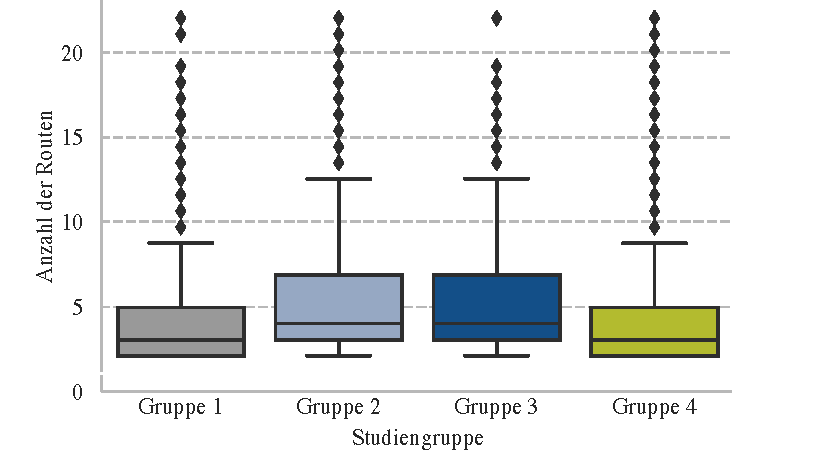
\includegraphics[width=\textwidth]{contents/06_model_evaluation/02_evaluation/res/usage_result_overview.pdf}
    \caption{Anzahl der gefahrenen Routen für jede Studiengruppe}
    \label{fig:evaluation_usage_result_overview}
\end{figure}

\autoref{fig:evaluation_usage_result_overview} enthält eine Übersicht der Verteilung der Anzahl der gefahrenen Routen pro Nutzer für jede Studiengruppe. Für die weitere Analyse wurden zunächst Ausreißer herausgefiltert. Dabei wurden alle Datenpunkte, welche mehr als dreimal die Standardabweichung vom Mittelwert entfernt sind aus dem Datensatz genommen. Final sind 3~951 Nutzer im Datensatz für die Prüfung der Hypothesen verblieben. Daraus sind die in \autoref{tab:study_usage_results} aufgelisteten Ergebnisse berechnet worden.

Zur Prüfung der Signifikanz wird wieder der Kruskal-Wallis-Test eingesetzt, da auch die Anzahl der gefahrenen Routen pro Studienteilnehmer nicht normalverteilt ist (Shapiro-Wilk: $ p = 0.0000 $). Mit $ p = 1.146748e-16 $ als Ergebnis der Kruskal-Wallis-Tests kann davon ausgegangen werden, dass ein Haupteffekt vorliegt.

\begin{table}[htb!]
    \centering
    \begin{tabular}{p{.27\textwidth}p{.27\textwidth}p{.35\textwidth}}
        \hline
        Studiengruppe  & Mittelwert [N] & Standardabweichung [N] \\
        \toprule
        Gruppe 1                & 3.2672 & 3.2958 \\
        Gruppe 2                & 3.2256 & 3.1961 \\
        Gruppe 3                & 4.6630 & 4.7043 \\
        Gruppe 4                & 4.5391 & 4.1509 \\
        \bottomrule
    \end{tabular}
    \caption{Übersicht der Ergebnisse der gefahrenen Routen der Nutzer}
    \label{tab:study_usage_results}
\end{table}

Für die Prüfung zwischen welchen Studiengruppen ein signifikanter Unterschied vorliegt, wird der Dunn-Test \cite{dunn1964multiple} verwendet, welcher die Signifikanz der Unterschiede zwischen den Studiengruppen berechnet. Die Prüfung ergibt, dass jeweils ein signifikanter Effekt zwischen den Gruppen 3 und 4 gegenüber den Gruppen 1 und 2 vorliegt ($ p_{13} = 6.242309e-10 $, $ p_{14} = 5.054949e-09 $, $ p_{23} = 2.491232e-09 $ $ p_{24} = 1.484581e-08 $). Folglich kann abgeleitet werden, dass die Nutzer NUNAV häufiger verwenden, wenn sie \textit{Context}-abhängige Erklärungen erhalten, unabhängig davon, ob diese kombiniert mit den statischen Erklärungen erfolgen. Folglich erfüllen nur die \textit{Context}-abhängigen Erklärungen die Anforderung NFR1.

Die Hypothesen 2.1 und 2.2 müssen abgelehnt werden, da weder alle Erklärungstypen zu einer signifikant häufigeren Nutzung von NUNAV führen, noch das Geben von beiden vorgestellten Typen von Erklärungen zu einer erhöhten Nutzung pro Studienteilnehmer führt im Vergleich zur Präsentation von nur einem der integrierten Erklärungstypen. 

\subsubsection{Nutzerabweichungen von der vorgeschlagenen Route}

Im Folgenden wird die Anforderung NFR2 geprüft, welche fordert, dass die Nutzer weniger häufig von der vorgeschlagenen Route abweichen sollen. Zur Prüfung wurden wiederum zwei Hypothesen aufgestellt:

\begin{enumerate}
    \item[3.1] WENN der Teilnehmer Erklärungen erhält, DANN folgt er signifikant häufiger der vorgeschlagenen Route als wenn er keine erhält.
    \item[3.2] WENN der Teilnehmer nur eine der beiden vorgestellten Erklärungstypen erhält, DANN folgt er signifikant weniger häufig der vorgeschlagenen Route als wenn ihm beide Arten von Erklärungen präsentiert werden.
\end{enumerate}

\begin{figure}[htb!]
    \centering
    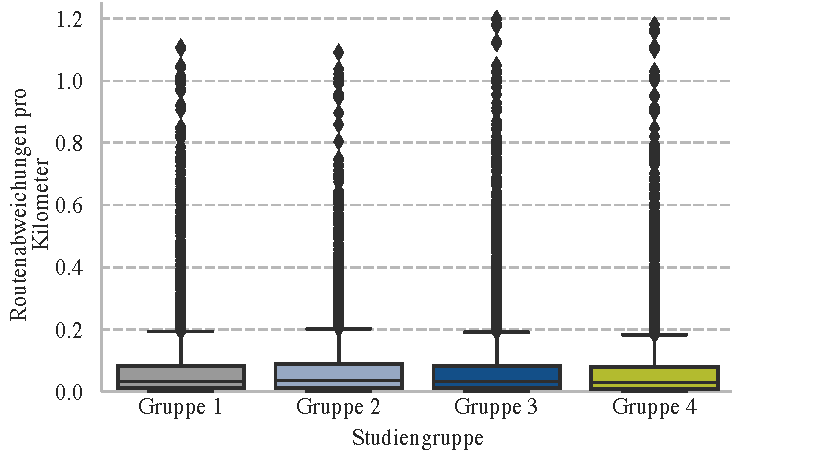
\includegraphics[width=\textwidth]{contents/06_model_evaluation/02_evaluation/res/off_route_result_overview.pdf}
    \caption{Anzahl der Abweichungen von der vorgeschlagenen Route pro Kilometer für jede Studiengruppe}
    \label{fig:evaluation_off_route_result_overview}
\end{figure}

Als Messwert wird die Anzahl der Abweichungen relativ zu Gesamtlänge der Route verwendet. Die Einheit ist Abweichungen pro Kilometer. Zu diesem Messwert, muss erwähnt werden, dass die Erkennung, wann Nutzer von der Route abweichen nicht trivial ist. Bei einer wirklichen Abweichung, wird dies in der Regel mehrfach gezählt und es kann generell schnell zu falsch positiven Messungen kommen. Aufgrund großen Datenmenge wird allerdings davon ausgegangen, dass diese Effekte einen vernachlässigbaren Effekt haben. Bei der Betrachtung von Abweichungen von der Route werden außerdem, wie zuvor beschrieben, Navigationen, bei denen es häufig zu einer ungenauen Positionierung kommt aus den Daten herausgefiltert. Außerdem wurden auch hier Ausreißer in den Daten mit der gleichen Bedingung wie zuvor herausgefiltert, sodass schlussendlich 16~314 einzelne Navigationen zur Analyse der Routen-Abweichungen im Datensatz verblieben sind. Die Daten für jede Studiengruppe sind in \autoref{fig:evaluation_off_route_result_overview} dargestellt. Die berechneten Ergebnisse sind in \autoref{tab:study_offroute_results} zusammengefasst.

\begin{table}[htb!]
    \centering
    \begin{tabular}{p{.27\textwidth}p{.27\textwidth}p{.35\textwidth}}
        \hline
        Studiengruppe  & Mittelwert [N/km] & Standardabweichung [N/km]\\
        \toprule
        Gruppe 1                & 0.0753 & 0.1293 \\
        Gruppe 2                & 0.0786 & 0.1272 \\
        Gruppe 3                & 0.0803 & 0.1410 \\
        Gruppe 4                & 0.0732 & 0.1328 \\
        \bottomrule
    \end{tabular}
    \caption{Übersicht der Ergebnisse der Routen-Abweichungen pro Kilometer}
    \label{tab:study_offroute_results}
\end{table}

Da auch die Daten der Routenabweichugen nicht normalverteilt sind (Shapiro-Wilk-Test: $ p = 0.0 $), wird zur Signifikanzprüfung der Kruskal-Wallis-Test verwendet \cite{wohlin2012experimentation}. Aufgrund des Ergebnisses von $ p = 0.000007 < 0.05 $, wird abgeleitet, dass ein Haupteffekt vorliegt. Es wird wieder mit dem Dunn-Test die Signifikanz zwischen den einzelnen Studiengruppen geprüft. 

Auch hier wird wieder von einem Signifikanzniveau $ p < 0.05 $ ausgegangen (Daten siehe \nameref{ch:appendix_1}). Folglich weichen die Nutzer der Gruppe 4 signifikant weniger von der vorgeschlagenen Route ab, als die Teilnehmer aller anderen Gruppen ($ p_{11} = 0.028808 $, $ p_{12} = 0.000003 $, $ p_{13} = 0.002962 $). Weitere signifikante Unterschiede gibt es nicht.

Hypothese 3.1 trifft zwar für das Geben aller Erklärungstypen (Gruppe 4) zu, nicht aber für die Gruppen 2 und 3. Folglich wird diese abgelehnt. Hypothese 3.2 kann angenommen werden, da die Nutzer der Gruppe 4 sowohl signifikant weniger von der vorgeschlagenen Route abgewichen sind als die Nutzer der Gruppe 2 sind als auch die Nutzer der Gruppe 3.

Zusammenfassend kann die Anforderung NFR2 durch das Geben von allen Erklärungen erfüllt werden. Einzelne Erklärungen weisen keinen signifikant positiven Effekt auf die Anzahl der Abweichungen von der Route auf. 

\subsubsection{Nutzerzufriedenheit mit der aktuellen Route}

Um die Zufriedenheit der Nutzer mit der abgeschlossenen Navigation zu evaluieren, setzt NUNAV auf eine Bewertung mithilfe von 5 Sternen bei Erreichen des Zieles. Dies ist verknüpft mit der Frage \glqq Wie hat dir die Fahrt gefallen?\grqq{} (siehe \autoref{fig:screenshot_destination_reached}). Außerdem sind die Fahrtdauer und zurückgelegte Kilometer angegeben. Die folgenden konkreten Hypothesen wurden für die Analyse abgeleitet:

\begin{enumerate}
    \item[4.1] WENN Teilnehmer Erklärungen erhalten, DANN geben sie im Vergleich eine signifikant höhere Bewertung für die Navigation ab, als wenn sie keine Erklärungen erhalten.
    \item[4.2] WENN Teilnehmer nur einen der beiden vorgestellten Erklärungstypen erhalten, DANN geben sie im Vergleich eine signifikant niedrigere Bewertung für die Navigation ab, als wenn sie beide Erklärungstypen erhalten.
\end{enumerate}

\begin{figure}[htb!]
    \centering
    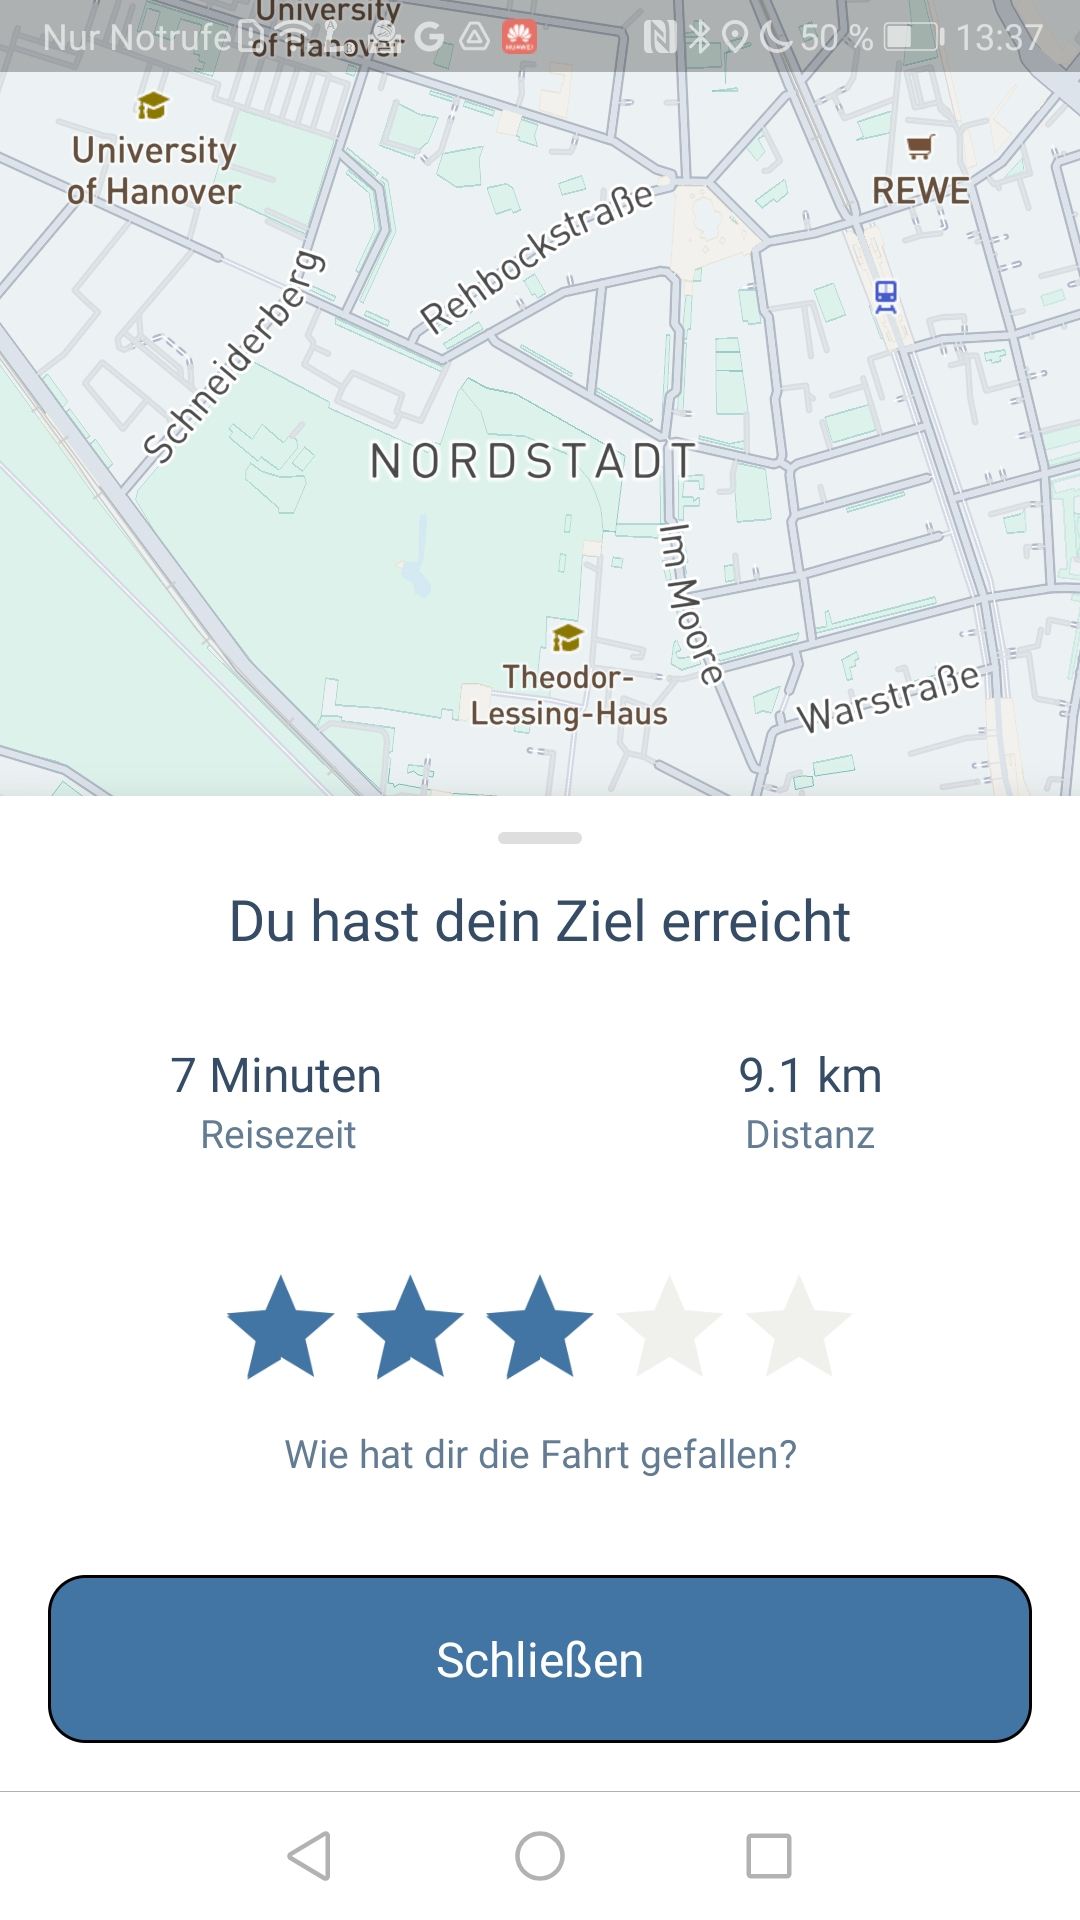
\includegraphics[width=0.27\textwidth]{contents/06_model_evaluation/02_evaluation/res/rating_screenshot.jpg}
    \caption{Bildschirmfoto des Bewertungsdialogs}
    \label{fig:screenshot_destination_reached}
\end{figure}


Für die Prüfung zwischen welchen Studiengruppen ein signifikanter Unterschied vorliegt, wird wieder der Dunn-Test \cite{dunn1964multiple} verwendet, nachdem ein Kruskal-Wallis-Test einen Haupteffekt zeigt ($ p = 0.00335 $). Daraus resultiert, dass es zwischen den Gruppen 1 und 3 ($ p = 0.005723$) sowie 3 und 4 ($ p = 0.024375 $) einen signifikanten Unterschied bei der Zufriedenheit mit der aktuellen Route gibt.

Mithilfe von \autoref{fig:Rating_Result_Overview} wird abgeleitet, dass es insbesondere mehr 5-Stern-Bewertungen in Gruppe 3 gegenüber den Gruppen 1 und 4 gibt. Die Anteile der ein und zwei Stern Bewertungen unterscheiden sich kaum. Folglich kann man sagen, dass die Teilnehmer signifikant zufriedener mit der Navigation waren, wenn sie Erklärungen wie in Gruppe 3 bekommen im Vergleich zu keinen Erklärungen (Gruppe 1) oder allen vorgestellten Erklärungstypen (Gruppe 4).

Da beim Geben von Erklärungen dies die Nutzerzufriedenheit nicht in jedem Fall erhöht, muss Hypothese 4.1 abgelehnt werden. Hypothese 4.2 muss ebenfalls abgelehnt werden, unter anderem da es einen gegenteiligen Effekt zwischen den Gruppen 3 und 4 gibt.

\begin{figure}[t!]
    \centering
    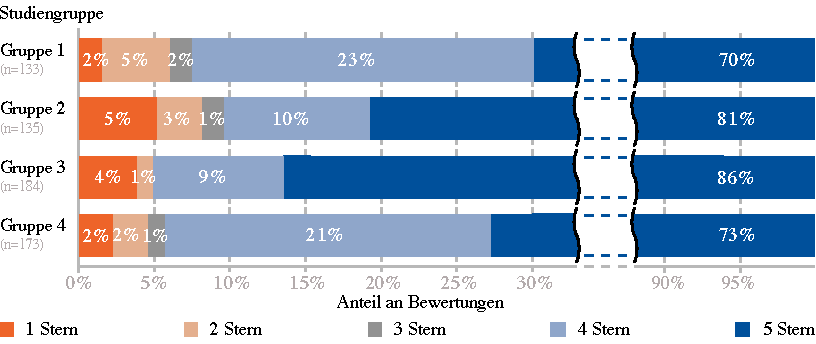
\includegraphics[width=\textwidth]{contents/06_model_evaluation/02_evaluation/res/rating_result_overview.pdf}
    \caption{Verteilung der Teilnehmer-Bewertung der Navigation für jede Studiengruppe bezogen auf die insgesamt abgegebenen Bewertungen}
    \label{fig:Rating_Result_Overview}
\end{figure}

\subsubsection{Zusammenfassung des Einflusses auf die externe Qualität}

Bei der Analyse der Einflüsse der Erklärungen, auf die externe Qualität von \textit{NUNAV Navigation}, dass die meisten Hypothesen abgelehnt werden müssen. Folglich fällt der Effekt der integrierten Erklärungen deutlich geringer aus, als zunächst erwartet. Positiv kann allerdings zusammengefasst werden, dass für keine Erklärung ein signifikant negativer Einfluss auf eine der Metriken gemessenen konnte.

Darüber hinaus gibt es einen positiven Effekt durch Erklärungen auf die Nutzung pro Woche und Nutzer, wenn die \textit{End User} \textit{Context}-abhängige Erklärungen erhalten. Sie nutzen NUNAV dann durchschnittlich 4,66 (\textit{Context}-abhängig + statisch) bzw. 4,54 (\textit{Context}-abhängig + statisch) mal pro Woche gegenüber 3,23 (statisch) bzw. 3,27 (keine Erklärung) mal pro Woche.

Die Anzahl der Routenabweichungen wird signifikant positiv (weniger) beeinflusst, wenn die \textit{End User} alle Erklärungen angezeigt bekommen (0,073 Abweichungen/km) gegenüber keinen Erklärungen (0,075 Abweichungen/km). 

Außerdem geben die \textit{End User} einen signifikant positivere Bewertung für die Route ab, wenn sie \textit{Context}-abhängige Erklärungen erhalten (durchschnittlich 4,73 Sterne vs. 4,55 Sterne). Hier gibt es allerdings scheinbar einen negativen Einfluss, wenn die \textit{End User} zusätzlich die statischen Erklärungen erhalten, da diese die Routen dann signifikant schlechter bewerten (durchschnittlich 4,6 Sterne).

Folglich erfüllen die \textit{Context}-abhängigen Erklärungen die Qualitätsanforderungen NFR1 und NFR3 und tragen somit zu einer signifikant häufigeren Nutzung von \textit{NUNAV Navigation} sowie mehr Zufriedenheit der \textit{End user} mit der Navigation bei. Folglich kann empfohlen werden, diese weiterhin in der Anwendung zu integrieren.

Für die statischen Erklärungen alleine kann kein signifikant positiver Effekt gemessen werden. Ein zusätzlich signifikant positiver Effekt im Rahmen von NFR2 (weniger Routenabweichungen) kann erreicht werden, wenn beide Erklärungstypen angezeigt werden. Allerdings hat dies zu einen negativen Effekt auf die Routen-Zufriedenheit der \textit{End User}, verglichen zum Einsatz von \textit{Context}-abhängigen Erklärungen. Für die statischen Erklärungen kann folglich keine klare Empfehlung zum Einsatz dieser aus der Case Study abgeleitet werden.

\newpage

\subsection{Direkte Evaluation der Erklärungen}
\label{sec:study_results_qualitativ}

Die zuvor analysierten Metriken betreffen ausschließlich die Auswirkungen von Erklärungen auf die \textit{Objectives} für die Integration - im konkreten Fall \textit{Usage Increase}, \textit{System Acceptance} und \textit{Satisfaction}.

\subsubsection{Ziel der direkten Evaluation}

Mithilfe der Metriken konnte überprüft werden, welche Erklärungen, in welchen Kombinationen den zuvor aufgestellten Anforderungen genügen. Es kann allerdings für die statischen Erklärungen keine Empfehlung abgeleitet werden, da diese insgesamt keine signifikant positiven Auswirkungen haben bzw. warum sowohl positive und negative Effekte im Vergleich zum ausschließlichen Einsatz der \textit{Context}-Erklärungen messbar sind. Folglich ist eine direkte Evaluation der Erklärungen nötig, wie sie auch im Leitfaden vorgeschlagen wird. Insbesondere wird dort empfohlen nicht nur Verhaltensmetriken, sondern auch qualitative Evaluationen von \textit{End Usern} zur Bewertung von Erklärungen zu nutzen. Daher ist im Anschluss an die 

Eine zweite Analyse soll zusätzliche Daten liefern, um die Ergebnisse Einflüsse der integrierten Erklärungen auf andere Qualitätsaspekte besser interpretieren zu können.

Das Ziel ist es folglich, konkrete Probleme oder Verbesserungspotential der entwickelten statischen Erklärungen aufzudecken.

\subsubsection{Methode}

Die direkte Analyse der Erklärungen ist wiederum in zwei Teile gegliedert. Zum einen wurden während der Case Study einige Meta-Daten gesammelt. Es wurde beispielsweise aufgezeichnet, wie viele der \textit{End User}, die die Möglichkeit hatten, auf die statische Erklärungen zuzugreifen, diese genutzt haben und wie lange, sie diese im Fokus hatten.

Um qualitative Aussagen zu den Erklärungen zu erhalten wurde außerdem ein Quasi-Experiment durchgeführt. Bei diesem wurden vier Studienteilnehmern jeweils alle vier Erklärungen gezeigt bzw. sie haben mit diesen interagiert. Im Anschluss an jede Erklärung wurden ihnen die gleichen Aussagen zur Bewertung auf einer Likert-Skala vorgelegt. Diese entsprechen den im Leitfaden unter Evaluation vorgestellten Aussagen (siehe \autoref{sec:model_evaluation}). Das heißt mithilfe der Aussagen zu den Erklärungen werden die Qualitätsaspekte \textit{Satisfaction}, \textit{Perceived Transparency}, \textit{Persuasiveness}, \textit{Usefulness}, und \textit{Completeness} der Erklärungen bewertet. Darüber hinaus wurden Aussagen zum Bedarf der jeweiligen Erklärung hinzugefügt.

Außerdem wurden die Teilnehmer gebeten, alle Gedanken beim Interagieren oder Lesen der Erklärungen mitzuteilen. Abschließend zu jeder Erklärung haben alle Teilnehmer außerdem die Möglichkeit erhalten Verbesserungsvorschläge für die Erklärungen zu machen oder auf fehlende Informationen in der Erklärung hinzuweisen. Der vollständige Fragebogen mit dem Ablauf des Quasi-Experiments ist in \nameref{ch:appendix_1} zu finden.

\subsubsection{Bedarf für die gegebenen Erklärungen}

Die statischen Erklärungen (siehe \autoref{sec:user_count_definition} und \autoref{sec:route_explanation_definition}), welche die Einflüsse auf den Routing-Algorithmus von NUNAV sowie das kollaborative Routing erklären, sind interaktiv. Somit kann evaluiert werden, wie viele Studienteilnehmer diese wie häufig diese angefordert haben. Außerdem kann gemessen werden, wie lange sie die Erklärungen betrachtet haben.

Die drei verschiedenen Erklärungen, die die Nutzer aufrufen können, sind in \autoref{sec:user_count_definition} und \autoref{sec:route_explanation_definition} beschrieben. Die Studiengruppen (Gruppe 2 und 4), denen diese angezeigt wurden, enthalten insgesamt 1~766 Teilnehmer.

Im Folgenden wird die Erklärung zu Einflüssen auf die Routenberechnung \textit{Erklärung 1}, die kurze Erklärung zum kollaborativen Routing als \textit{Erklärung 2.1} und die dazugehörige weitere Erklärung als \textit{Erklärung 2.2} genannt.

Als erfasst und nicht direkt wieder verlassen werden die Erklärungen gewertet, wenn die \textit{End User} länger als 1,5 Sekunden in dem Dialog verbracht haben \cite{BAHR2011776}. \autoref{fig:explanation_results_clicked} zeigt wie häufig die \textit{End User} die Erklärungen erfasst haben. 

\begin{figure}[htb!]
    \centering
    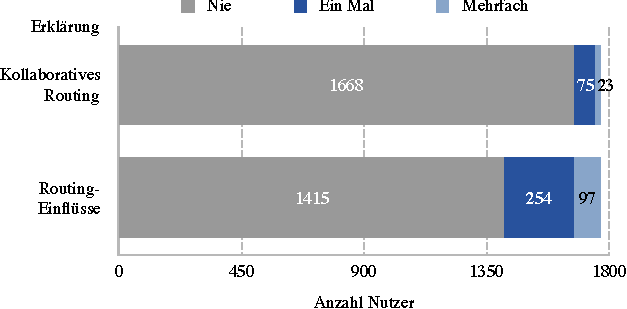
\includegraphics[width=0.9\textwidth]{contents/06_model_evaluation/02_evaluation/res/explanation_results_clicked.pdf}
    \caption{Anzahl der Nutzer, die Erklärungen erfasst haben}
    \label{fig:explanation_results_clicked}
\end{figure}


\autoref{fig:evaluation_explanation_demand_qualitative} zeigt die Bewertung der Studienteilnehmer des Quasi-Experiments in Bezug auf deren Bedarf für die Erklärungen.

In \autoref{fig:explanation_results_clicked} kann man erkennen, dass etwa 5\% der Nutzer auf die Erklärung zum kollaborativen Routing geklickt haben. Allerdings sagen wie in \autoref{fig:evaluation_explanation_demand_qualitative} zu erkennen ist drei von vier Teilnehmern des Quasi-Experiments, dass die die Erklärung benötigt haben. Folglich herrscht eine Diskrepanz zwichen dem wirklichen Bedarf und den \textit{End Usern} des Feld Tests, die die Erklärung angefordert haben. Insbesondere haben im Quasi-Experiment zwei der Teilnehmer angegeben, die Erklärung sich auch mehrfach anzusehen.

% TODO: Ich möchte Ausblenden können und empfand als störend mit in die Grafik einfügen. Ggf. doch Grafiken teilen

\begin{figure}[htb!]
    \centering
    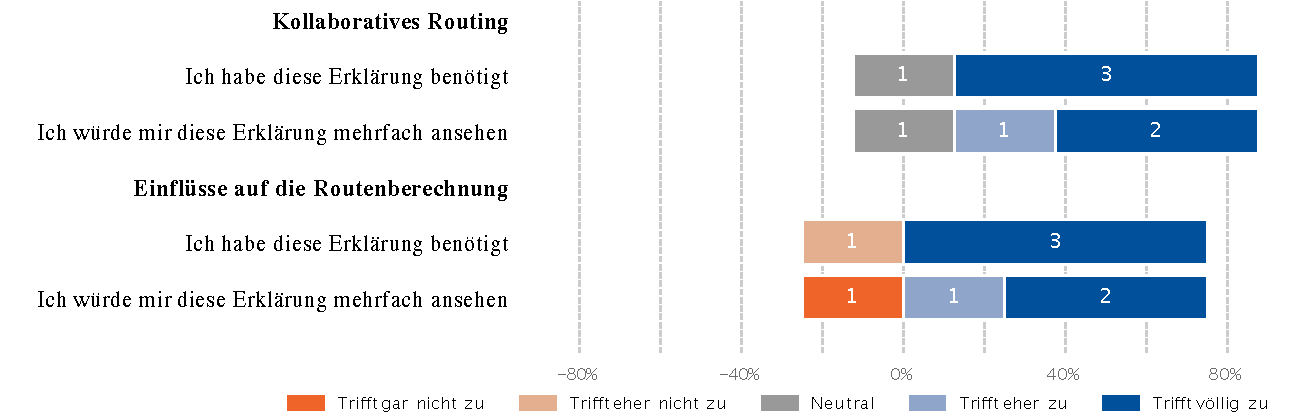
\includegraphics[width=\textwidth]{contents/06_model_evaluation/02_evaluation/res/qualitativeFeedback-evaluation_explanation_demand_qualitative.pdf}
    \caption{Subjektive Einschätzung des Bedarfs der Erklärungen}
    \label{fig:evaluation_explanation_demand_qualitative}
\end{figure}

Betrachtet man im Gegensatz dazu die gleichen Daten für die Erklärung zu den Einflüssen auf die Routenberechnung fällt auf, dass etwa 20\% der Teilnehmer des Feldtests sich die Erklärung angesehen haben, wie in \autoref{fig:evaluation_explanation_demand_qualitative} zu sehen aber, sowohl weniger Teilnehmer angegeben haben, dass sie die Erklärung benötigt haben als auch sich mehrfach ansehen würden als bei der Erklärung zum kollaborativen Routing. Ein Erklärungsversuch kann durch die Aussage eines Teilnehmers am Quasi-Experiment getätigt werden. Dieser sagte, dass die Zahl, auf die für die kollaborative Routing Erklärung geklickt werden müsse, zum Teil klar ist und nicht direkt offensichtlich ist, dass sich dort hinter die ALgorithmuserklärung befinde. Außerdem hat eine Teilnehmerin hinzugeügt, dass die Frage \glqq Wie ist meine Route entstanden?\grqq{}, über welche die Erklärung zu den Routing-Einflüssen erreichbar ist neugieriger macht.

Aus diesen freien Aussagen und dem Gegensatz zwischen den benötigten Erklärungen und den wirklich angeforderten, kann folglich abgeleitet werden, die Erklärung zum kollaborativen Routing offensichtlicher zu erreichen sein sollte. Die Idee eines weiteren Teilnehmers war, dass es Möglich sein sollte, diese Erklärung über den Dialog \glqq Trete Schwarm bei...\grqq{} erreichen zu können. Dies ist der Dialog, der zu sehen ist, während \textit{NUNAV Navigation} die erste Route während der Nutzung lädt.

Außerdem kann es dadurch, dass nur bis zu 20\% der \textit{End User} in der Feldstudie die Erklärungen gelesen haben, sein, dass die Auswirkungen auf andere Qualitätsmerkmale in der Studie nicht im signifikanten Bereich lagen. Zumindest für die Erklärung zum kollaborativen Routing ließe sich dies anhand der Aussagen der Teilnehmer des Quasi-Experiments durch einen verbesserten Weg, um zur Erklärung zu gelangen, ggf. steigern und sollte in einer zweiten Iteration getestet werden. Des Weiteren gab es in einem Fall beim Quasi-Experiment Kritik daran, dass die Hilfe-Center-Artikel im Browser des Smartphones geöffnet würden. Eine Integration in die App würde der Aussage nach eher dazu bewegen, sich eine Erklärung auch durchzulesen.

Für die beiden \textit{Context-Abhängigen} Erklärungen gab es keine Metriken, welchen den Bedarf innerhalb der Feld-Studie widerspiegeln können. Auch gab es im Rahmen des Quasi-Experiments lediglich positive Rückmeldungen zum Bedarf der Erklärungen. Auch wurden beide Erklärungen weder als störend empfunden, noch gab es Studienteilnehmer, die den Wunsch geäußert haben, die Erklärungen ausblenden zu wollen (siehe \nameref{ch:appendix_1}).

\subsubsection{Nützlichkeit der gegebenen Erklärungen}

\autoref{tab:explanation_results_clicked} zeigt die Bewertung als \glqq Hilfreich\grqq{} oder \glqq Nicht hilfreich\grqq{} durch die Nutzer. Allerdings sind die Hilfe-Artikel auch über andere Wege erreichbar, wodurch Bewertungen nicht nur von Nutzern kommen, die über die NUNAV-App dort hingeleitet wurden.

\begin{table}[htb!]
    \centering
    \begin{tabular}{p{.5\textwidth}p{.15\textwidth}p{.25\textwidth}}
        \hline
        Artikel & Hilfreich & Nicht Hilfreich \\
        \toprule
        Kollaboratives Routing & 76 & 9 \\
        Einflüsse auf die Routenberechnung & 209 & 32 \\
        \bottomrule
    \end{tabular}
    \caption{\textit{Usefulness} der Hilfe-Center-Artikel}
    \label{tab:explanation_results_clicked}
\end{table}

\begin{figure}[htb!]
    \centering
    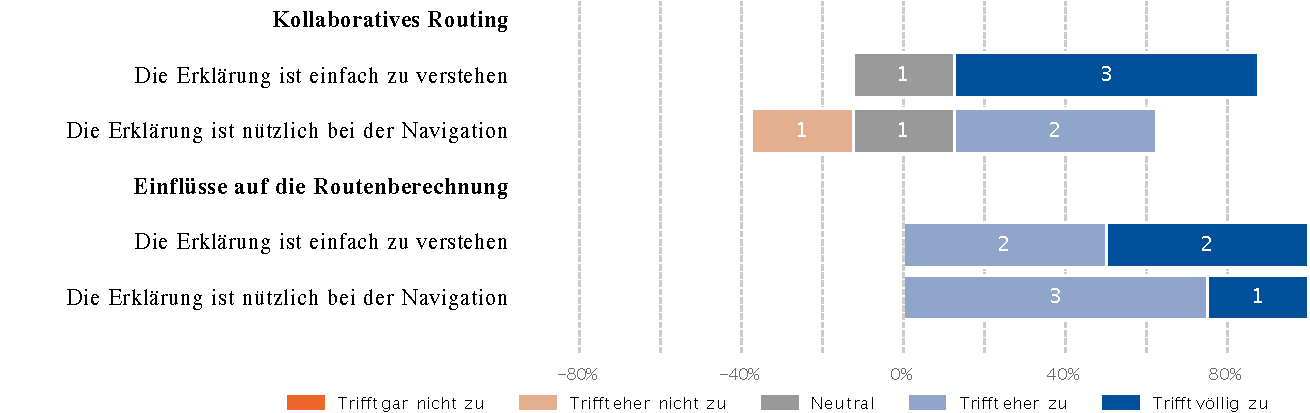
\includegraphics[width=\textwidth]{contents/06_model_evaluation/02_evaluation/res/qualitativeFeedback-evaluation_usefulness_qualitative.pdf}
    \caption{Subjektive Einschätzung des Bedarfs der Erklärungen (Anzahl der jeweiligen Bewertung pro Aussage)}
    \label{fig:evaluation_usefulness_qualitative}
\end{figure}

\newpage

\subsubsection{Erklärung: Kollaboratives Routing}

\begin{figure}[htb!]
    \centering
    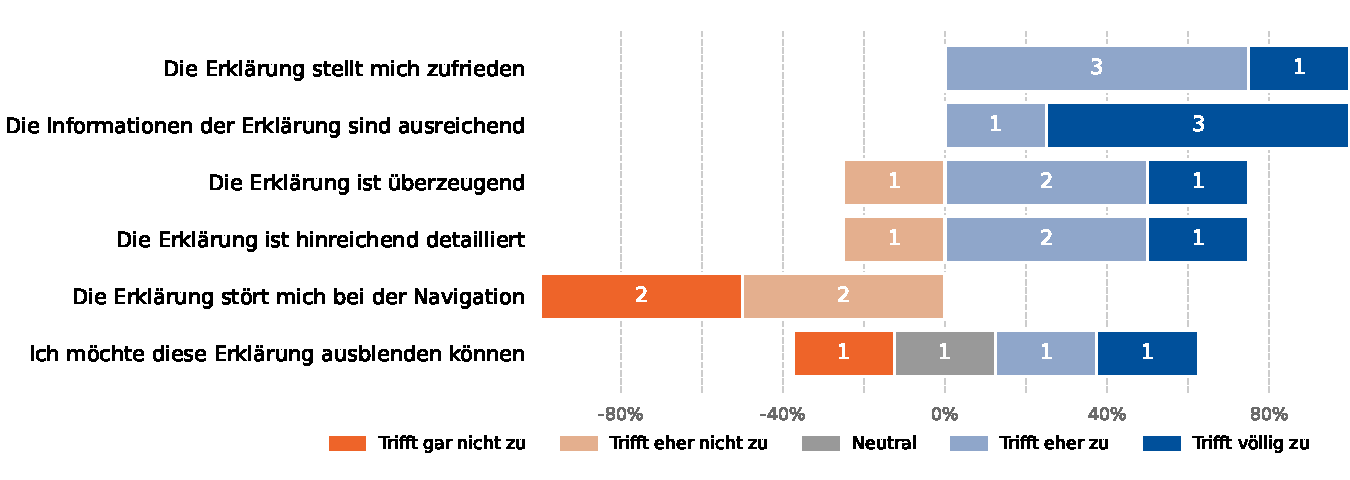
\includegraphics[width=\textwidth]{contents/06_model_evaluation/02_evaluation/res/qualitativeFeedback-01_collaborative_routing_short.pdf}
    \caption{Anzahl der jeweiligen Bewertung pro Aussage für die Erklärung zu kollaborativem Routing}
    \label{fig:01_collaborative_routing_short}
\end{figure}

\subsubsection{Erklärung: Einflüsse auf die Routenberechnung}

\begin{figure}[htb!]
    \centering
    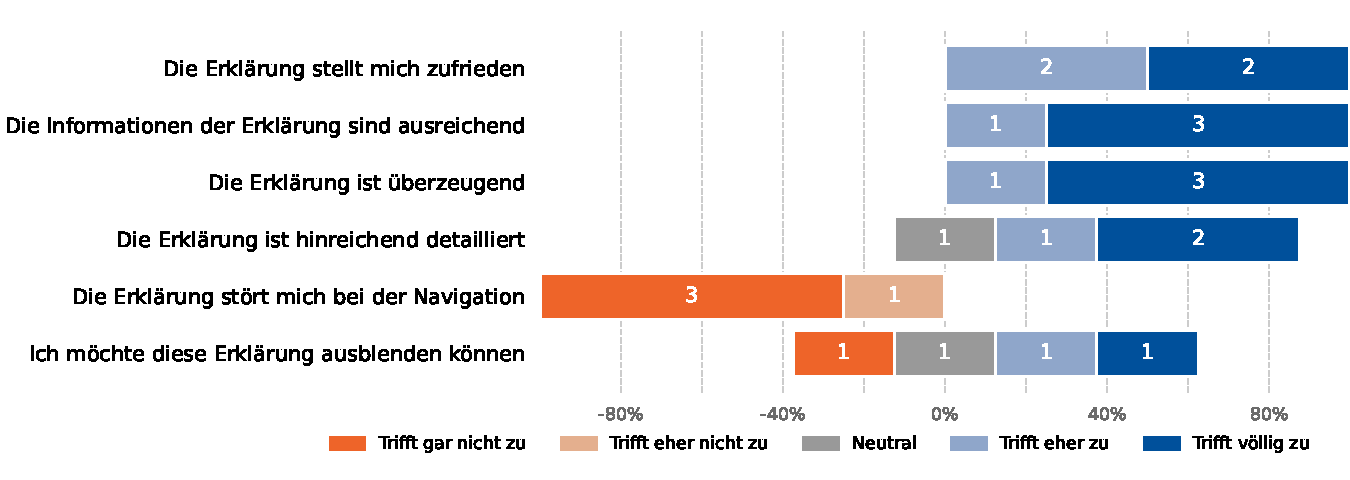
\includegraphics[width=\textwidth]{contents/06_model_evaluation/02_evaluation/res/qualitativeFeedback-02_collaborative_algorithm_short.pdf}
    \caption{Anzahl der jeweiligen Bewertung pro Aussage für die Erklärung zu Einflüssen auf die Routenberechnung}
    \label{fig:02_collaborative_algorithm_short}
\end{figure}


\subsubsection{Erklärung: Verkehrsaufkommen}


\subsubsection{Erklärung: Positionsungenauigkeiten}

\subsection{Zusammenfassung der Evaluation}

Mit einer \textit{Case Study} innerhalb der Produktivversion von \textit{NUNAV Navigation} wurden zunächst die Qualitätsanforderungen von Graphmasters an die Einflüsse der integrierten Erklärungen untersucht. Dies hat ergeben, dass die Erklärung zum kollaborativen Routing sowie zum zu den Einflüssen auf den Routingalgorithmus keinen signifikanten Effekt auf die Metriken für die aufgestellten Anforderungen (siehe \autoref{sec:explanation_requirements}) haben.

Als positives Ergebnis der \textit{Case Study} kann hervorgehoben werden, dass die Erklärungen zum aktuellen Verkehrsgeschehen und zu Positionsungenauigkeiten während der Navigation einen positiven Einfluss auf die \textit{Route Satisfaction} der \textit{End User} haben. Außerdem konnte gezeigt werden, dass \textit{End User}, die diesen Erklärungstyp erhalten im Vergleich zu jenen, die keine oder nur die statischen Erklärungen erhalten haben \textit{NUNAV Navigation} im Durchschnitt pro Woche häufiger zur Navigation verwenden.

Außerdem zeigt die Analyse der \textit{Case Study}, dass das Geben aller Erklärungstypen ein signifikant positiven Effekt auf die \textit{Route Acceptance} hat, allerdings im Vergleich zum Geben nur der \textit{Context}-Abhängigen Erklärungen ein signifikant negativer Einfluss auf die \text{Route Satisfaction} messbar ist.

Aufgrund der mangelnden Ergebnisse zu den Eigenschaften der entwickelten Erklärungen wurde im Anschluss eine Quasi-Experiment durchgeführt, welches zusammen mit weiteren Metadaten aus der \textit{Case Study} für die beiden statischen Erklärungen potentielle Verbesserungen herausgestellt hat.

Dies ist auch ein möglicher Einflussfaktor, dass durch die statischen Erklärungen alleine keine signifikanten Ergebnisse in der durchgeführten \textit{Case Study} für die gemessen Qualitätsaspekte festgestellt werden konnten.

Für die \textit{Context}-Abhängigen Erklärungen konnten keine konkreten Vorschläge oder Ergebnisse aus dem Quasi-Experiment gefolgert werden. Dies hat allerdings die Qualität der Erklärungen, welche aus der \textit{Case Study} gefolgert wurde bestätigt.

Als Konsequenz sollten die in \autoref{sec:demand_qualitative_evaluation} erfolgten Vorschläge der Teilnehmer des \textit{Quasi-Experiments} in eine zweite Iteration der Erklärungen integriert werden. Eine weitere Evaluation kann im Anschluss feststellen, ob die Hypothese, dass die vorgeschlagenen Verbesserungen zu den in den Anforderungen geforderten messbaren Erfolgen führt, angenommen werden kann.

